\section{三阶段 作用}

Pre-prepare phase 和 Prepare phase (预准备和准备阶段) 用于确保所有节点在同一视图 (view) 下，并能够对请求进行全局排序，即使负责提议请求排序的主节点 (primary) 出现故障时也能保持一致性。

\begin{figure}[htbp]
\centering
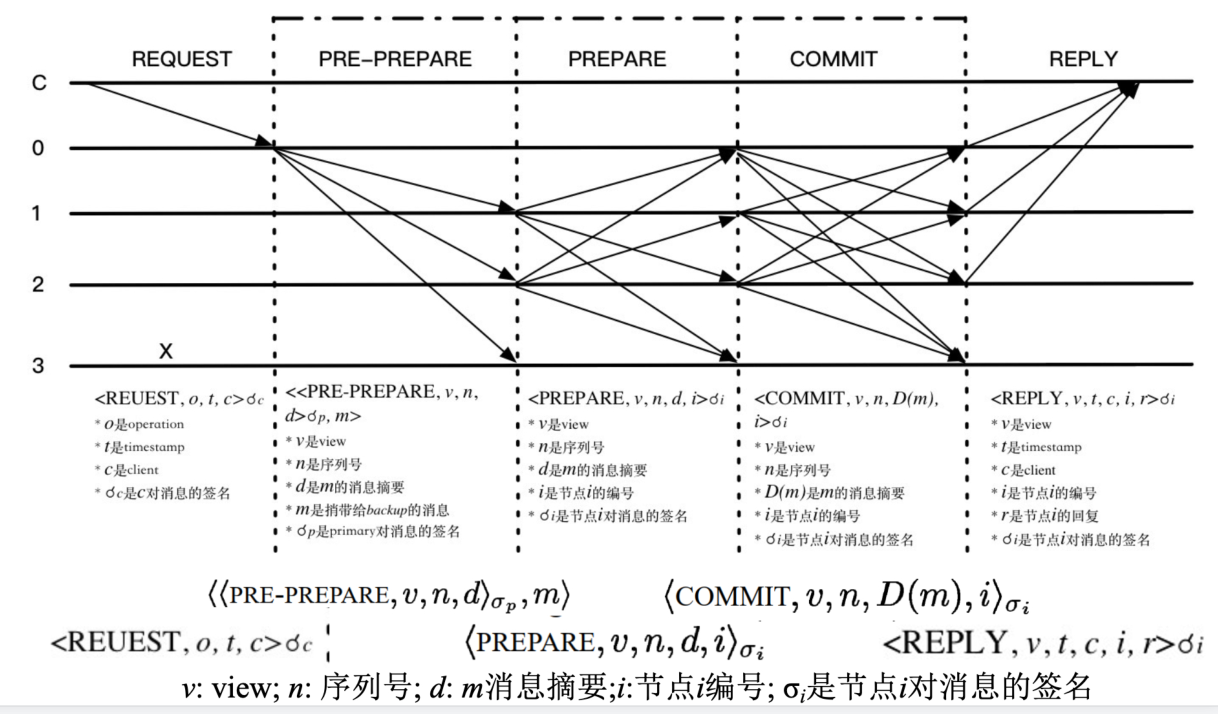
\includegraphics[width=0.8\textwidth]{figures/ch9/ch9_pbft_preprepare_prepare.png}
\caption{PBFT Pre-prepare 与 Prepare 阶段消息流程}
\end{figure}

\begin{table}[htbp]
  \centering
  \begin{tabular}{ccccc}
    \toprule
    & & 提交消息 [疑似: 给部分节点提交] & & \\
    \midrule
    节点 = & 1. 给所有节点广播正确的; 2. 给所有节点广播错误的; 3. 给部分节点广播错误的 & & \textasciitilde{} & 注意节点不切换 \\
    \bottomrule
  \end{tabular}
\end{table}

\subsection{View-change 阶段 (视图切换阶段)}

\begin{itemize}
  \item 有恶意节点 (最多 $f$ 个) 频繁发起视图切换
  \item 该进行视图切换时，恶意节点不切换
  \item 触发: 各节点只要收到 $f+1$ 个 View\_Change，自己便也发出 View\_Change。
  \item 达成: 新的主节点只要收到 $2f+1$ 个 View\_Change，即可发出 New\_View。
\end{itemize}

\subsection{PBFT 对比 Paxos}

\begin{itemize}
  \item PBFT 对比 Paxos，最大的不同在于解决的问题不一样
  \begin{itemize}
    \item 虽然都是共识算法，但一个解决的是拜占庭问题
    \item 另一个则解决的是非拜占庭问题
  \end{itemize}
  \item PBFT 中对应的主节点可能为恶意节点
  万一主节点作恶，从节点要有发现其是恶意节点的能力；
  并及时通过视图更换协议更换主节点
  \item BFT 需要从节点与从节点的消息交互
  只听主节点肯定是不行的，还要看看其他节点的意见；
  才有足额的节点认为是对的，就同意。
  \item 算法耗资源方面
  \begin{itemize}
    \item 明显 PBFT 要更复杂，投票数明显多
    \item [疑似: 内存占用、带宽开销更大]；
  \end{itemize}
  相比之下，[疑似: 其他共识算法(如 Paxos/ZAB) 在 PBFT 面前开销更小]。
\end{itemize}

\subsection{总结 PBFT 优点 vs. 缺点}

\subsubsection{优点:}

\begin{itemize}
  \item 首个实用的 BFT 共识容错算法，使得复杂度从指数级降低到多项式级 $O(n^2)$；
  \item 响应性 (Responsiveness): 在网络状况 OK，主节点不犯错，拜占庭节点数量不超过 $f$ 个时，在下一个视图一定是可以达成共识的。
\end{itemize}

\subsubsection{缺点:}

\begin{itemize}
  \item 通信复杂度 $O(n^2)$，可扩展性低；
  \item 视图转换的复杂度 $O(n^3)$，若考虑主节点和拜占庭节点，视图转换复杂度 $O(f n^3)$；
  \item 视图转换期间只能接收 view\_change、new\_view 消息，不能对外提供服务；
  \item Safety 和 Liveness 属性需要通过视图转换来保障。
\end{itemize}

\begin{figure}[htbp]
\centering
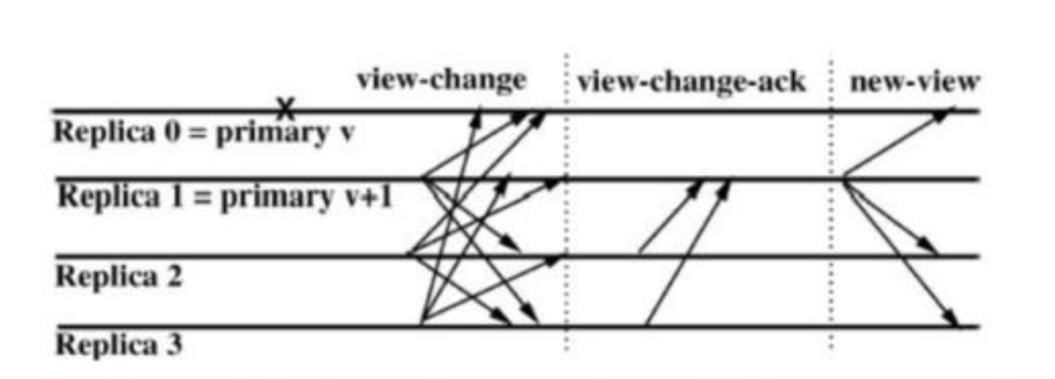
\includegraphics[width=0.8\textwidth]{figures/ch9/ch9_pbft_view_change.png}
\caption{PBFT View-change 视图切换协议}
\end{figure}

\begin{figure}[htbp]
\centering
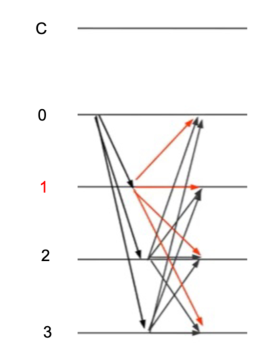
\includegraphics[width=0.8\textwidth]{figures/ch9/ch9_pbft_vs_paxos.png}
\caption{PBFT 与 Paxos 对比}
\end{figure}

% 图片：<!-- image -->，请替换实际路径
%\includegraphics[width=0.8\textwidth]{../work/figures/placeholder}

% 图片：<!-- image -->，请替换实际路径
%\includegraphics[width=0.8\textwidth]{../work/figures/placeholder}

\subsection{End of PBFT}
